\documentclass{beamer}
\setbeamertemplate{caption}[numbered]
\usepackage{graphicx}
\usepackage{svg}
\usepackage[utf8]{inputenc}
\usepackage[english]{babel}
\graphicspath{{Graphs/}}
\usepackage{comment}
\usepackage{verbatim}
\usepackage{hyperref}
\mode<presentation>
{
	\usetheme{AnnArbor}
	\usecolortheme{crane}
}

\title[Model Interpretation and Visualization I]{Model Interpretation and Visualization I Supplemental}
\subtitle[ISRC Workshop]{Iowa Social Research Center (ISRC) Workshop}
\author[Wallace \& LaCombe]{Desmond D. Wallace \& Scott J. LaCombe}
\institute[University of Iowa]{Department of Political Science\\The University of Iowa\\Iowa City, IA}

\date{October 24, 2018}

\begin{document}

\begin{frame}
 \titlepage
\end{frame}

\section{OLS Marginal Effects}

\begin{frame}
	\frametitle{OLS Marginal Effects Definitions}
		\begin{itemize}
			\item Measuring the change in the dependent variable for a change in one independent variable, holding remaining independent variables constant.
				\begin{itemize}
					\item \textit{Marginal Change} is the partial derivative, or instantaneous rate of change, in the dependent variable w.r.t. an independent variable, holding remaining variables constant.
					\item \textit{Discrete Change} is the difference in the prediction from one specified value of an independent variable to another specified value, holding remaining variables constant.
				\end{itemize}
		\end{itemize}
\end{frame}

\begin{frame}
	\frametitle{OLS Marginal Effects Formulas}
		\begin{itemize}
			\item Marginal Change: $\frac{\partial E[Y|X]}{\partial x_{k}}=\frac{\partial X\beta}{\partial x_{k}}=\beta_{k}$
			\item Discrete Change: $\frac{\Delta E[Y|X]}{\Delta x_{k}\left(x^{start}_{k}\rightarrow x^{end}_{k}\right)}=E[Y|X, x^{end}_{k}]-E[Y|X, x^{start}_{k}]$
		\end{itemize}
\end{frame}

\begin{frame}
	\frametitle{OLS Marginal Effects Interpretations}
		\begin{itemize}
			\item $\frac{\partial E[Y|X]}{\partial x_{k}}=\frac{\Delta E[Y|X]}{\Delta x_{k}\left(x^{start}_{k}\rightarrow x^{end}_{k}\right)}=\beta_{k}$ when $x^{start}_{k}\rightarrow x^{end}_{k}=1$, assuming there is no interaction terms.
			\item The standard error of the marginal effect is the same as the standard error of the estimated beta coefficient.
			\item \textit{For a unit increase in $x_{k}$, the expected change in $Y$ equals $\beta_{k}$, holding all other variables constant.}
			\item \textit{Having characteristic $x_{k}$ (as opposed to not having the characteristic) results in an expected change of $\beta_{k}$ in $Y$, holding all other variables constant.}
		\end{itemize}
\end{frame}

\begin{frame}
	\frametitle{OLS Marginal Effects}
		\begin{figure}[p]
			\centering
			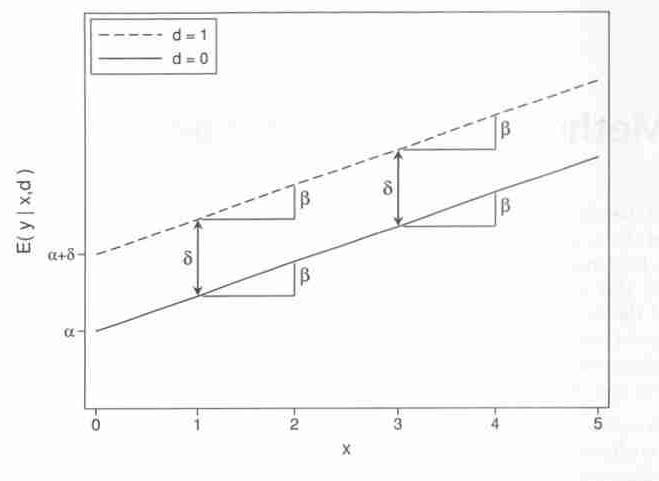
\includegraphics[scale=0.45]{images/ols_marginal_effects.png}
			\label{fig:fig1}
		\end{figure}
\end{frame}

\section{BRM Marginal Effects}

\begin{frame}
	\frametitle{BRM Marginal Effects Definitions}
		\begin{itemize}
			\item Measuring the change in the probability of an outcome for a change in one independent variable, holding remaining independent variables constant at specific values.
				\begin{itemize}
					\item \textit{Marginal Change} is the rate of change in the probability for an infinitely small change in $x_{k}$, holding other variables at specific values.
					\item \textit{Discrete Change} is the actual change in the predicted probability for a given change in $x_{k}$, holding other variables at specific values.
				\end{itemize}
		\end{itemize}
\end{frame}

\begin{frame}
	\frametitle{BRM Marginal Effects Formulas}
		\begin{itemize}
			\item Marginal Change: 
				\begin{itemize}
					\item General: $\frac{\partial Pr\left(y=1|X=x^{*}\right)}{\partial x_{k}}=f(X\beta)\beta_{k}$
						\begin{itemize}
							\item Probit -- $f=\mbox{Normal PDF}$
							\item Logit -- $f=\mbox{Logistic PDF}$
						\end{itemize}
					\item Logit only: $\frac{\partial Pr\left(y=1|X=x^{*}\right)}{\partial x_{k}}=Pr\left(y=1|X=x^{*}\right)\left[1-Pr\left(y=1|X=x^{*}\right)\right]\beta_{k}$
				\end{itemize}
			\item Discrete Change: $\frac{\Delta Pr\left(y=1|X=x\right)}{\Delta x_{k}\left(x^{start}_{k}\rightarrow x^{end}_{k}\right)}=Pr\left(y=1|X=x, x_{k}=x^{end}_{k}\right)-Pr\left(y=1|X=x, x_{k}=x^{start}_{k}\right)=F(X\beta, x_{k}=x^{end}_{k})-F(X\beta, x_{k}=x^{start}_{k})$
				\begin{itemize}
					\item Probit -- $F=\mbox{Normal CDF}$
					\item Logit -- $F=\mbox{Logistic CDF}$
				\end{itemize}
		\end{itemize}
\end{frame}

\begin{frame}
	\frametitle{BRM Marginal Effects Interpretation}
		\begin{itemize}
			\item $\frac{\partial Pr\left(y=1|X=x^{*}\right)}{\partial x_{k}}\approx\frac{\Delta Pr\left(y=1|X=x\right)}{\Delta x_{k}\left(x^{start}_{k}\rightarrow x^{end}_{k}\right)}$, the more linear the probability curve is in the region where the change is occurring.
			\item In general, $\frac{\partial Pr\left(y=1|X=x^{*}\right)}{\partial x_{k}}\neq\frac{\Delta Pr\left(y=1|X=x\right)}{\Delta x_{k}\left(x^{start}_{k}\rightarrow x^{end}_{k}\right)}$
		\end{itemize}
\end{frame}

\begin{frame}
	\frametitle{BRM Marginal Effects}
		\begin{figure}[p]
			\centering
			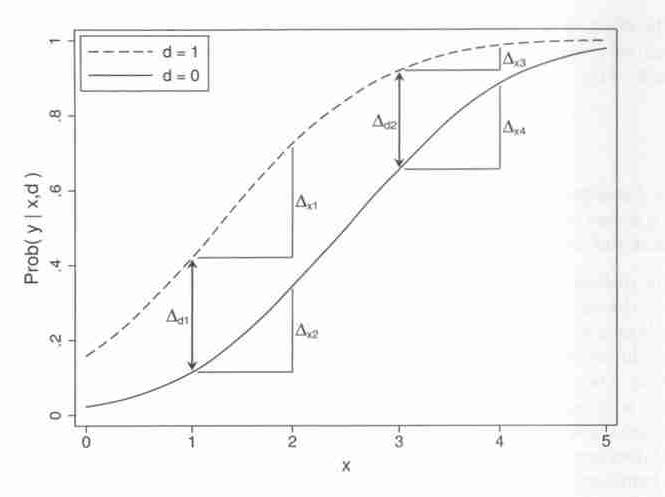
\includegraphics[scale=0.45]{images/brm_marginal_effects.png}
			\label{fig:fig2}
		\end{figure}
\end{frame}

\begin{frame}
	\frametitle{BRM Marginal Effects Types}
		\begin{itemize}
			\item Average Marginal Effect (AME) -- The marginal effect of $x_{k}$ for each observation at its observed values $x_{i}$, and taking the average of these effects.
				\begin{itemize}
					\item Marginal Change
						\begin{itemize}
							\item $\frac{1}{N}\sum_{i=1}^{N}\frac{\partial Pr\left(y=1|X=x_{i}\right)}{\partial x_{k}}$
							\item \textit{The average marginal effect of $x_{k}$ is...}
						\end{itemize}
					\item Discrete Change
						\begin{itemize}
							\item $\frac{1}{N}\sum_{i=1}^{N}\frac{\Delta Pr\left(y=1|X=x_{i}\right)}{\Delta x_{k}\left(x^{start}_{k}\rightarrow x^{end}_{k}\right)}$
							\item \textit{On average, increasing $x_{k}$ by $\delta$ increases the probability by...}
							\item \textit{On average, increasing $x_{k}$ from \underline{start-value} to \underline{end-value} increases the probability by...}
						\end{itemize}
				\end{itemize}
		\end{itemize}
\end{frame}

\begin{frame}
	\frametitle{BRM Marginal Effects Types}
		\begin{itemize}
			\item Marginal Effect at the Mean (MEM) -- The marginal effect of $x_{k}$ with all independent variables held at their means.
				\begin{itemize}
					\item Marginal Change
					\begin{itemize}
						\item $\frac{\partial Pr\left(y=1|X=\bar{x_{k}}\right)}{\partial x_{k}}$
						\item \textit{For someone who is average on all characteristics, the marginal change of $x_{k}$ is...}
					\end{itemize}
				\item Discrete Change
					\begin{itemize}
						\item $\frac{\Delta Pr\left(y=1|X=\bar{x_{k}}\right)}{\Delta x_{k}\left(x^{start}_{k}\rightarrow x^{end}_{k}\right)}$
						\item \textit{For someone who is average on all characteristics, increasing $x_{k}$ by $\delta$ changes the probability by...}
					\end{itemize}
			\end{itemize}
		\end{itemize}
\end{frame}

\begin{frame}
	\frametitle{BRM Marginal Effects Types}
		\begin{itemize}
			\item Marginal Effect at Representative Values (MER) -- The marginal effect of $x_{k}$ with independent variables held at specific values.
				\begin{itemize}
					\item Specify values that are instructive for the substantive questions under consideration.
					\item MEM is a special case of MER.
					\item If not all variables are specified, MERs will be calculated for the variables specified, and averaged across the values for the unspecified variables.
				\end{itemize}
		\end{itemize}
\end{frame}

\begin{frame}
	\begin{center}
		\begin{LARGE}
			Email: desmond-wallace@uiowa.edu\\
			Any Questions?
		\end{LARGE}
	\end{center}
\end{frame}

\end{document}
